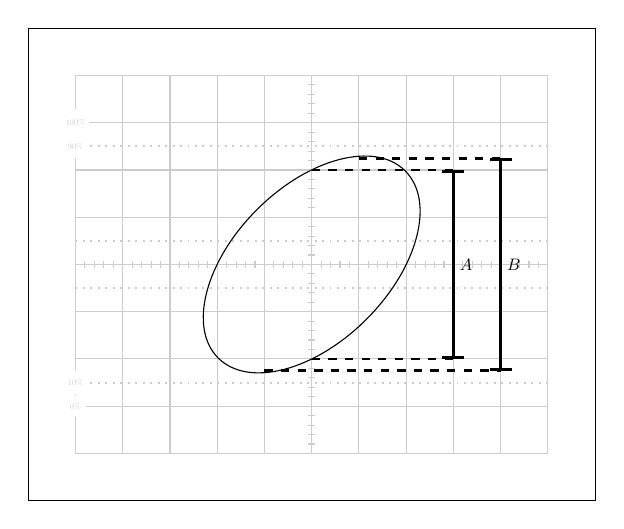
\begin{tikzpicture}[scale=0.6,every node/.style={transform shape}]
\def\scalTa{0.02};%EscalaTemporal señal 1
\def\scalTb{0.02};%EscalaTemporal señal 2
\def\scalVa{1};%EscalaVertical señal 1
\def\scalVb{1};%EscalaVertical señal 2
\def\offseta{0};%Nivel de offset de la señal señal 1
\def\offsetb{0};%Nivel de offset de la señal señal 2

%Lineas intermedias grilla
\foreach \x in {-5,-4.8,...,4.8,5}{
    \draw[gray!40,thin,shift={(\x,0)}] (0pt,2pt) -- (0pt,-2pt);
}
\foreach \y in {-4,-3.8,...,3.8,4}{
    \draw[gray!40,thin,shift={(0,\y)}] (2pt,0pt) -- (-2pt,0pt);
}
\foreach \a [evaluate={\y=\a*0.5}] in {-5,-1,1,5}{
    \draw[gray!40,line width=0.7pt,dotted] (-5,\y) -- (5,\y);
}

%Grilla
\draw[thin,gray!40] (-5,-4) grid (5,4);
\node[fill=white,text=gray!40,circle,scale=0.5] at (-5,3) {$100\%$};
\node[fill=white,text=gray!40,circle,scale=0.5] at (-5,2.5) {$90\%$};
\node[fill=white,text=gray!40,circle,scale=0.5] at (-5,-2.5) {$10\%$};
\node[fill=white,text=gray!40,circle,scale=0.5] at (-5,-3) {$0\%$};
\draw[black] (-6,-5) rectangle(6,5);

\draw[rotate=-45] (0, 0) ellipse (0.82cm*2 and 1.4cm*2);
\draw[line width=1pt,dashed](0,2)--(3,2);
\draw[line width=1pt,dashed](0,-2)--(3,-2);
\draw[line width=1pt,|-|](3,2)--(3,-2) node[midway,right]{$A$};
\draw[line width=1pt,dashed](1,2.25)--(4,2.25);
\draw[line width=1pt,dashed](-1,-2.25)--(4,-2.25);
\draw[line width=1pt,|-|](4,2.25)--(4,-2.25) node[midway,right]{$B$};
\end{tikzpicture}
\caption*{Modo X-Y}